\chapter{Neuronale Netzwerke}

Unter einem neuronalen Netzwerk versteht man ein System
aus Neuronen. Diese sind schichtweise organisiert wobei
jedes Neuron einer Schicht jeweils zu allen Neuronen der
direkt anliegenden Schichten verbunden ist.
Abbildung \ref{fig:Neuronales Netzwerk} zeigt beispielhaft ein
neuronales Netzwerk aus 19 Neuronen mit insgesamt 5 Schichten.\bigskip

\begin{figure}[h]
    \begin{center}
        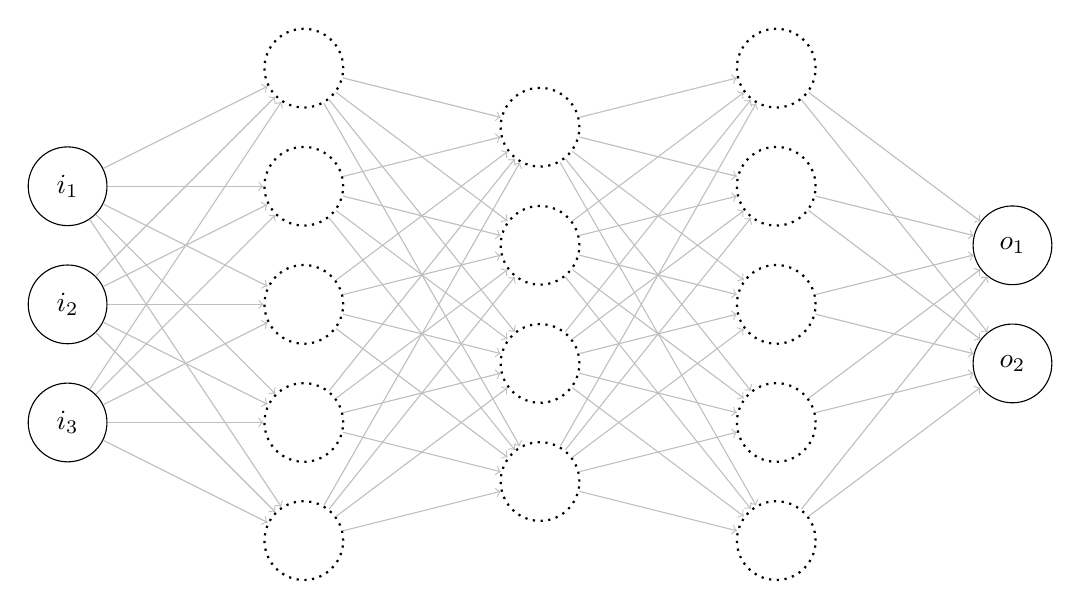
\begin{tikzpicture}[y=-1.5cm,x=3cm]
            \tikzset{
                netnode/.style={circle,draw=black,minimum size=1cm},
                hidden/.style={dotted,thick}
            }
            \node[netnode] (i1) at (0,0) {$i_1$};
            \node[netnode] (i2) at (0,1) {$i_2$};
            \node[netnode] (i3) at (0,2) {$i_3$};

            \node[netnode,hidden] (l11) at (1,-1) {};
            \node[netnode,hidden] (l12) at (1,0) {};
            \node[netnode,hidden] (l13) at (1,1) {};
            \node[netnode,hidden] (l14) at (1,2) {};
            \node[netnode,hidden] (l15) at (1,3) {};

            \node[netnode,hidden] (l21) at (2,-0.5) {};
            \node[netnode,hidden] (l22) at (2,0.5) {};
            \node[netnode,hidden] (l23) at (2,1.5) {};
            \node[netnode,hidden] (l24) at (2,2.5) {};

            \node[netnode,hidden] (l31) at (3,-1) {};
            \node[netnode,hidden] (l32) at (3,0) {};
            \node[netnode,hidden] (l33) at (3,1) {};
            \node[netnode,hidden] (l34) at (3,2) {};
            \node[netnode,hidden] (l35) at (3,3) {};

            \node[netnode] (o1) at (4,0.5) {$o_1$};
            \node[netnode] (o2) at (4,1.5) {$o_2$};

            \foreach \i in {1,2,3}{
                    \foreach \j in {1,...,5}{
                            \draw[->,black!25] (i\i) -- (l1\j);
                        }
                }
            \foreach \i in {1,...,5}{
                    \foreach \j in {1,...,4}{
                            \draw[->,black!25] (l1\i) -- (l2\j);
                        }
                }
            \foreach \i in {1,...,4}{
                    \foreach \j in {1,...,5}{
                            \draw[->,black!25] (l2\i) -- (l3\j);
                        }
                }
            \foreach \i in {1,...,5}{
                    \foreach \j in {1,2}{
                            \draw[->,black!25] (l3\i) -- (o\j);
                        }
                }
        \end{tikzpicture}
    \end{center}
    \caption{Struktur eines neuronalen Netzwerks}
    \label{fig:Neuronales Netzwerk}
\end{figure}

\section{Neuronen}\label{sec:neurons}

Unter einem Neuron versteht sich in neuronalen Netzen lediglich ein Knoten,
in dem üblicherweise eine 32-Bit Zahl hinterlegt ist. Die Semantik
dieses Wertes hängt von dem jeweiligen Typ der Schicht ab, in dem sich das
Neuron befindet.
Die Werte aller Neuronen, mit Ausnahme jener aus der Eingabeschicht, setzen sich
aus den Werten aller Neuronen der direkt davor liegenden Schicht zusammen.
Das genaue Vorgehen bei der Wertermittlung hängt vom Entwurf des Netzwerks
und den dort verwendeten Aktivierungsfunktionen ab.

\section{Schichten und Kanten}\label{sec:layers}

In einem neuronalen Netzwerk ist jedes Neuron einer Schicht mit allen Neuronen
der jeweils davor liegenden und danach liegenden Schichten über Kanten verbunden.
Neuronale Netzwerke sind unidirektionale Graphen, demnach fließen Informationen
über Schichten (und folglich Kanten) nur in eine Richtung.

Die Kanten eines Netzwerks sind gewichtet, welche initial netzwerkabhängig
generiert, manuell zugewiesen oder durch zuvor erlernte Daten bestimmt werden.
Beim Trainieren eines Netzwerks werden diese in jeder Lerniteration
(auch \emph{Epoch} genannt) justiert, während sie im Betrieb keine Änderungen
mehr erfahren.
Der Entwurf eines Netzwerks bestimmt die Performanz dessen und die damit
verbundenen Hardwareanforderungen, nicht jedoch die Genauigkeit.
Diese wird überwiegend von den Kantengewichten bestimmt, daher ist das Ziel
des Trainings diese zu optimieren und damit die Genauigkeit des Netzwerks bei
gleicher Performanz zu erhöhen. Der Unterschied zwischen einem genauen und
einem ungenauen Netzwerk ist daher oft nur das investierte Training.

Kantengewichte wirken sich maßgeblich auf die Werteberechnung von Neuronen aus.
Diese wird in zwei Schritten ausgeführt. Im ersten Schritt wird aus den
Kantengewichten aller eingehenden Kanten und den Werten der darüber
verbundenen Neuronen die Produktsumme gebildet.
Für den zweiten Schritt sind jeweils Aktivierungsfunktionen notwendig, welche
im nachfolgenden Kapitel erläutert werden.

\section{Aktivierungsfunktionen}\label{sec:activation}

Im zweiten Schritt wird die zuvor bestimmte Produktsumme durch eine Funktion
modifiziert. Sogenannte \emph{Aktivierungsfunktionen} können beliebig gewählt
werden, müssen jedoch offensichtlich alle möglichen Eingaben auf einen Wert
abbilden können. Aktivierungsfunktionen erwarten genau einen Eingabewert
und bilden diesen auf genau einen Wert ab. Ein einfaches Beispiel ist die
Identitätsfunktion $\text{id}(x) = x$. Die eingesetzten Aktivierungsfunktionen
können schichtweise variieren. Einmal gewählt sind diese jedoch für das
entworfene Netzwerk fest.

Diese beiden Berechnungsschritte werden schichtweise in Richtung des
Datenflusses des Netzwerks für alle Neuronen durchgeführt. Im folgenden
Beispiel wird bildhaft dargestellt, wie solch eine Neuronenwertberechnung für
ein Netzwerk aussieht, welche in der betrachteten Schicht die
$tanH$-Aktivierungsfunktion verwendet.\bigskip

\begin{figure}
    \centering
    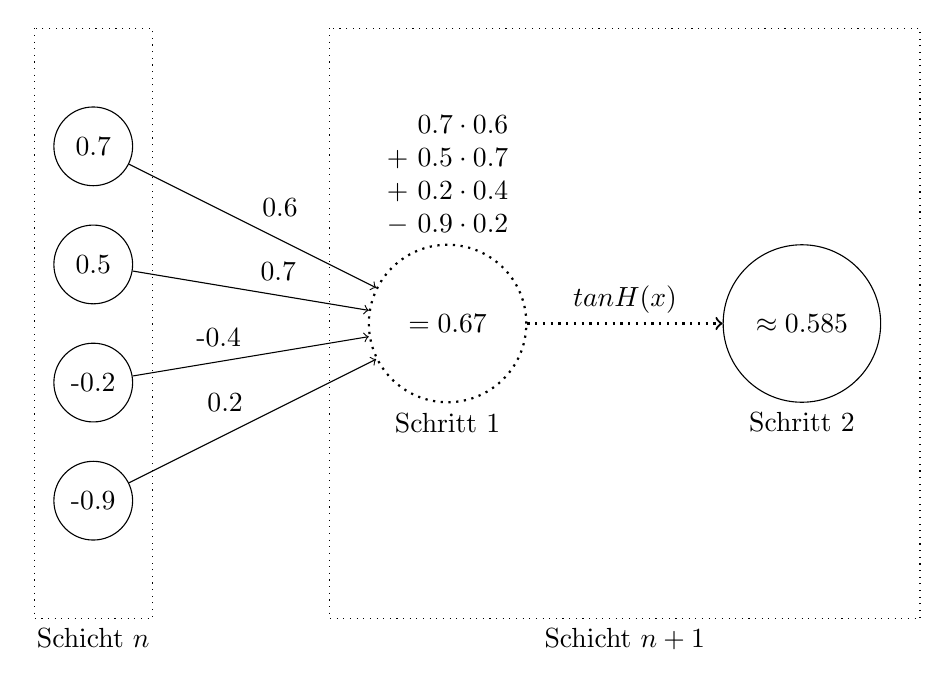
\begin{tikzpicture}[y=-1.5cm,x=1.5cm]
        \tikzset{
            netnode/.style={circle,draw=black,minimum size=1cm},
            hidden/.style={dotted,thick}
        }
        \node[netnode] (i1) at (0,0) {0.7};
        \node[netnode] (i2) at (0,1) {0.5};
        \node[netnode] (i3) at (0,2) {-0.2};
        \node[netnode] (i4) at (0,3) {-0.9};

        \draw[draw=black,dotted] (-0.5,-1) rectangle ++(1,5) ++(-0.5,0) node[below] {Schicht $n$};
        \draw[draw=black,dotted] (2,-1) rectangle ++(5,5) ++(-2.5,0) node[below] {Schicht $n+1$};

        \node[netnode,minimum size=2cm,dotted,thick] (o1) at (3,1.5) [label=below:Schritt 1] {$=0.67$};
        \node (o1l) [above of=o1,align=right,above] {$0.7\cdot 0.6$\\$+\ 0.5\cdot 0.7$\\$+\ 0.2\cdot 0.4$\\$-\ 0.9\cdot 0.2$};

        \node[netnode,minimum size=2cm] (o2) at (6,1.5) [label=below:Schritt 2] {$\approx 0.585$};

        \draw[->] (i1) -- node[auto] {0.6} (o1);
        \draw[->] (i2) -- node[auto] {0.7} (o1);
        \draw[->] (i3) -- node[auto] {-0.4} (o1);
        \draw[->] (i4) -- node[auto] {0.2} (o1);
        \draw[->,dotted,thick] (o1) -- node[above] {$tanH(x)$} (o2);
    \end{tikzpicture}
    \caption{Berechnung eines Neuronenwertes\\mit der $tanH$ Aktivierungsfunktion}
\end{figure}

Die Wahl der Aktivierungsfunktion beeinflusst die möglichen
Werte, die Neuronen im Netzwerk annehmen können. Um eine
Wertexplosion zu vermeiden (z.B. bei Verwendung von $ReLU(x): \max(0,x)$ als
Aktivierungsfunktion), können Normalisierungsschichten verwendet
werden, dessen Aufgabe die Einschränkung von Neuronenwerten auf einen
erwünschten Zielbereich ist. Es existieren jedoch auch Aktivierungsfunktionen,
die diese sogenannte \emph{Squashing-}Eigenschaft direkt besitzen. Darunter
zählt auch die im vorherigen Beispiel verwendetete Funktion $tanH$, bei der
alle Eingaben auf den Zielbereich [-1,1] abgebildet werden.

Im Folgenden sind sind einige Aktivierungsfunktionen abgebildet, welche
üblicherweise in neuronale Netzwerken eingesetzt werden.\bigskip

\begin{figure}[H]
    \begin{minipage}{0.45\textwidth}
        \begin{center}
            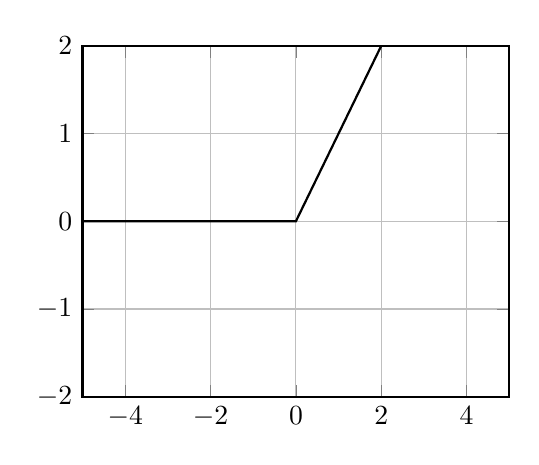
\begin{tikzpicture}
                \begin{axis}[width=7cm,xmin=-5,xmax=5,ymin=-2,ymax=2,thick,grid=both]
                    \addplot[] {max(x,0))};
                \end{axis}
            \end{tikzpicture}
        \end{center}
        \caption{ReLU}
    \end{minipage}\hfill
    \begin{minipage}{0.45\textwidth}
        \begin{center}
            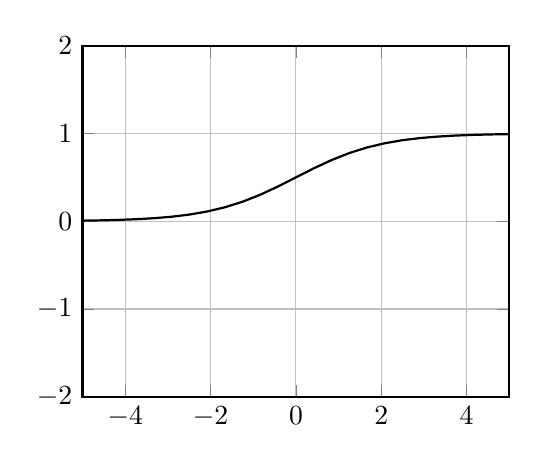
\begin{tikzpicture}
                \begin{axis}[width=7cm,xmin=-5,xmax=5,ymin=-2,ymax=2,thick,grid=both]
                    \addplot[] {1/(1+exp(-x))};
                \end{axis}
            \end{tikzpicture}
        \end{center}
        \caption{Sigmoid}
    \end{minipage}
\end{figure}
%
\begin{figure}[H]
    \begin{minipage}{0.45\textwidth}
        \begin{center}
            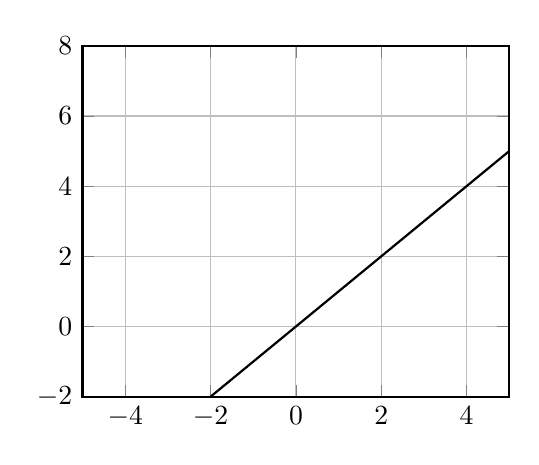
\begin{tikzpicture}
                \begin{axis}[width=7cm,xmin=-5,xmax=5,ymin=-2,ymax=8,thick,grid=both]
                    \addplot[] {x};
                \end{axis}
            \end{tikzpicture}
        \end{center}
        \caption{Softmax}
    \end{minipage}\hfill
    \begin{minipage}{0.45\textwidth}
        \begin{center}
            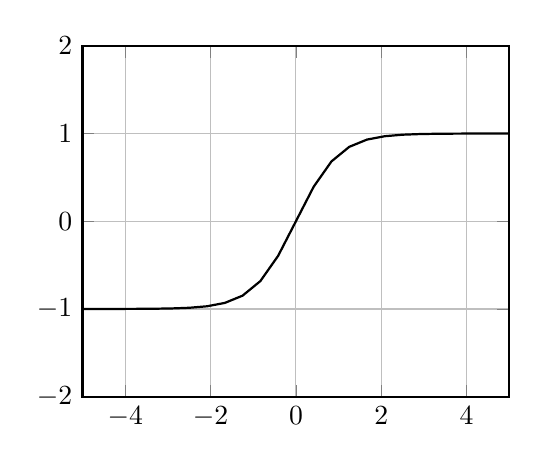
\begin{tikzpicture}
                \begin{axis}[width=7cm,xmin=-5,xmax=5,ymin=-2,ymax=2,thick,grid=both]
                    \addplot[] {(exp(x)-exp(-x)) / (exp(x)+exp(-x))};
                \end{axis}
            \end{tikzpicture}
        \end{center}
        \caption{tanH}
    \end{minipage}
\end{figure}

\section{Training}\label{sec:training}

Wie zuvor erwähnt, liegen die Stärken und Schwächen eines neuronalen Netzwerks
neben dem Aufbau und der Anzahl der verwendeten Schichten sowie der gewählten
Aktivierungsfunktionen vor allem in den Kantengewichten. Diese zu optimieren
kann ein langwieriger und rechenintensiver Prozess sein. Kleine Änderungen in
der Struktur des Netzwerks können große Teile von zuvor erlernten Gewichten
unbrauchbar machen, daher werden Netzwerke häufig an sich selbst trainiert.
Das bedeutet, dass beim Trainieren des Netzwerks die initialen
Kantengewichte keine emprischen Daten aus anderen (ähnlichen) Netzwerk verwenden,
selbst wenn beide Netzwerke auf dem identischen Datensatz trainiert werden.

\subsection{Ablauf}

Beim Training werden wiederholt unterschiedliche Eingaben in das Netzwerk gegeben,
zu denen die korrekten Klassifizierungen bekannt ist. In der letzten Schicht
des Netzwerks, der Ausgabeschicht, wird die vom Netzwerk bestimmte
Klassifizierung mit der tatsächlichen Klassifizierung verglichen.
Konkret werden die vom Netzwerk bestimmten Neuronenwerte in der Ausgabeschicht
mit den erwarteten Werten verglichen. Die absolute Differenz dieser Werte wird
als Fehler bezeichnet.
Beim Training wird diese Information in jedem Durchlauf verwendet, um die
Kantengewichte so anzupassen, dass der Fehler verringert, oder im
Optimalfall ganz zu eliminiert wird (Fehler = 0).
In der folgenden Abbildung ist ein Beispiel einer Fehlerbestimmung dargestellt.\bigskip

\begin{figure}[H]
    \centering
    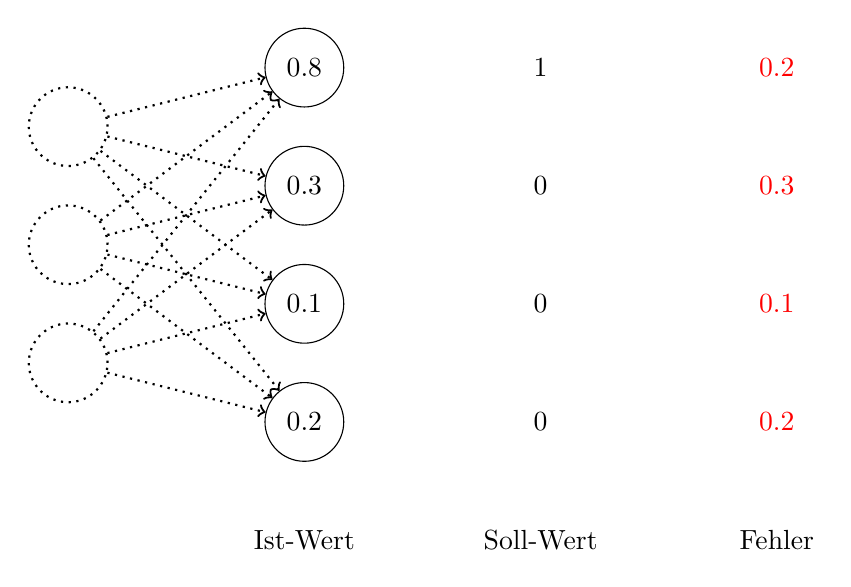
\begin{tikzpicture}[x=3cm,y=-1.5cm]
        \tikzset{
            netnode/.style={circle,draw=black,minimum size=1cm},
            hidden/.style={dotted,thick}
        }
        \node[netnode,hidden] (h1) at(0,0.5) {};
        \node[netnode,hidden] (h2) at(0,1.5) {};
        \node[netnode,hidden] (h3) at(0,2.5) {};

        \node[netnode] (o1) at (1,0) {0.8};
        \node[netnode] (o2) at (1,1) {0.3};
        \node[netnode] (o3) at (1,2) {0.1};
        \node[netnode] (o4) at (1,3) {0.2};

        \foreach \i in {1,2,3}{
                \foreach \j in {1,2,3,4}{
                        \draw[->,thick,dotted] (h\i) -- (o\j);
                    }
            }

        \node at (2,0) {1};
        \node at (2,1) {0};
        \node at (2,2) {0};
        \node at (2,3) {0};

        \node at (3,0) {\color{red}0.2};
        \node at (3,1) {\color{red}0.3};
        \node at (3,2) {\color{red}0.1};
        \node at (3,3) {\color{red}0.2};

        \node at (1,4) {Ist-Wert};
        \node at (2,4) {Soll-Wert};
        \node at (3,4) {Fehler};

    \end{tikzpicture}
\end{figure}

\subsection{Backpropagation}

Es stellt sich nun die Frage, ob und wie errechnet werden kann, welches
Kantengewicht wie angepasst werden muss, um den Fehler zu verringern.
Der Begriff der \emph{Backpropagation} beschreibt das Durchlaufen des Netzwerks,
jedoch entgegen der eigentlichen Laufrichtung und das Rückschließen der
notwendigen Gewichtsanpassung, um die Ausgabewerte der jeweiligen Lerneinheit
in die gewünschten Richtungen zu verändern.

Um eine Anpassung an einem Kantengewicht vorzunehmen, muss zuerst
festgestellt werden, wie die errechneten Fehler sich bei Änderungen an einem
bestimmten Gewicht verhalten. Dazu wird die sogenannte \emph{Slope} ermittelt,
eine Kurve auf der das Kantengewicht im Verhältnis zum Fehler steht.
Anschließend wird die Steigung dieser Kurve an der aktuellen Stelle, also
dem aktuellen Kantengewicht errechnet.
Offensichtlich lässt sich aus diesem Ergebnis, in welche Richtung das Kantengewicht
justiert werden muss um den Fehler zu verringern.
Ein Beispiel dazu befindet sich in der folgenden Abbildung. Dort ist die Tangente
der Fehlerkurve an der Stelle -0.5 in rot dargestellt.
Eine Erhöhung des Kantengewichts führt demnach zu einer Verringerung des
gemessenen Fehlers.\bigskip

\begin{figure}[H]
    \centering
    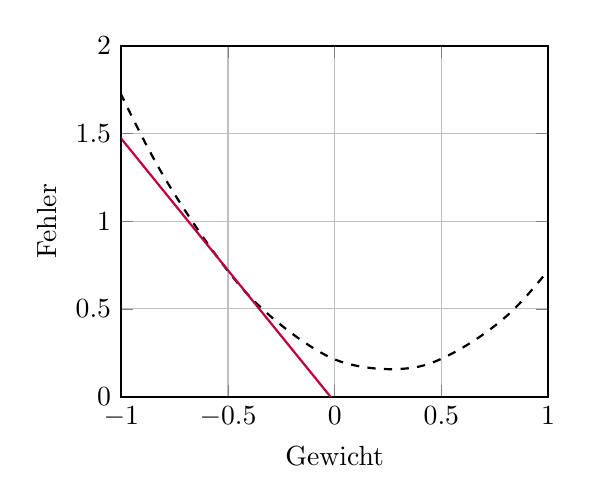
\begin{tikzpicture}
        \begin{axis}[xlabel=Gewicht,ylabel=Fehler,width=7cm,xmin=-1,xmax=1,ymin=0,ymax=2,thick,grid=both]
            \addplot[dashed,smooth] {(x-0.25)^2+0.15};
            \addplot[draw=purple] {-1.5*x-0.03};
        \end{axis}
    \end{tikzpicture}
\end{figure}

Diese Anpassungen werden in jeder Trainingseinheit für alle Kantengewichte
durchgeführt. Die Bestimmung der Stärke der Anpassung wird als Lernrate
bezeichnet.
Die Ermittlung der Fehlerkurve kann mathematisch durch das Verwenden der
sogenannten \emph{Chainingrule} \cite{Rumelhart} effizient ermittelt werden.
Zur Verbildlichung dieser Regel zeigt die folgende Abbildung
einen Ausschnitt aus einem einfachen neuronalen Netzwerk mit drei Schichten.\bigskip

\begin{figure}[H]
    \centering
    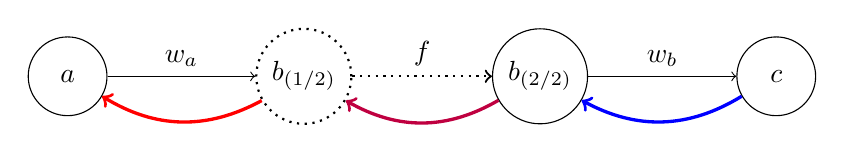
\begin{tikzpicture}[x=3cm]
        \tikzset{
            netnode/.style={circle,draw=black,minimum size=1cm},
        }
        \node[netnode] (a) at(0,0) {$a$};
        \node[netnode,dotted,thick] (b1) at(1,0) {$b_{(1/2)}$};
        \node[netnode] (b2) at(2,0) {$b_{(2/2)}$};
        \node[netnode] (c) at(3,0) {$c$};

        \draw[->] (a) -- node[above] {$w_a$} (b1);
        \draw[->,dotted,thick] (b1) -- node[above] {$f$} (b2);
        \draw[->] (b2) -- node[above] {$w_b$} (c);
        \draw[->,very thick,draw=blue] (c) to[bend left] (b2);
        \draw[->,very thick,draw=purple] (b2) to[bend left] (b1);
        \draw[->,very thick,draw=red] (b1) to[bend left] (a);
    \end{tikzpicture}
    \caption{Neuronenkette: Backpropagation}
\end{figure}

Die notwendige Anpassung des Kantengewichts $w_a$ zur Verringerung des Fehlers
in $c$ kann wie folgt ermittelt werden:

\[
    \frac{\delta c}{\delta w_a}=\color{red}\frac{\delta b_{(1/2)}}{\delta w_a}\color{purple}\cdot\frac{\delta b_{(2/2)}}{\delta b_{(1/2)}}\color{blue}\cdot\frac{\delta c}{\delta b_{(2/2)}}
\]

Diese Kette lässt sich weiter vereinfachen:

\begin{align*}
    \frac{\delta c}{\delta w_a} & = a\cdot\frac{\delta b_{(2/2)}}{\delta b_{(1/2)}}\cdot\frac{\delta c}{\delta b_{(2/2)}} & \left(\frac{\delta b_{(1/2)}}{\delta w_a} =a\right)                   \\
                                & = a\cdot f'(b_{(1/2)})\cdot\frac{\delta c}{\delta b_{(2/2)}}                            & \left(\frac{\delta b_{(2/2)}}{\delta b_{(1/2)}} =f'(b_{(1/2)})\right) \\
                                & = a\cdot f'(a\cdot w_a)\cdot\frac{\delta c}{\delta b_{(2/2)}}                           & \left(b_{(1/2)} =a\cdot w_a\right)                                    \\
                                & = a\cdot f'(a\cdot w_a)\cdot w_b                                                        & \left(\frac{\delta c}{\delta b_{(2/2)}} =w_b\right)                   \\
\end{align*}

Mit $a$, $w_a$ bekannt und $f'$ leicht ermittelbar wird auch deutlich, warum
die üblich verwendeten Aktivierungsfunktionen häufig stetig sind und einfach
abzuleiten sind.
Offensichtlich lässt sich dieses Vorgehen auf jede beliebig lange Neuronenkette
ausweiten und erlaubt somit die Ermittlung der Richtungen aller notwendigen
Gewichtsanpassungen zur Verringerung des Fehlers.
Im zuvor erwähnten Optimalfall wird jedes Kantengewicht solange angepasst,
bis ein Fixpunkt erreicht wurde und damit jedes Gewicht genau im Tal der
jeweiligen Fehlerkurve liegt. Das Erreichen dieses Tals kann erschwert werden,
wenn die verwendete Lernrate beim Training entweder zu hoch oder zu niedrig ist.
Daraus können zu starke oder zu schwache Anpassungen der Gewichte folgen.
Ersteres führt zum hin- und herspringen des ermittelten Gewichts auf der
Fehlerkurve sodass sich dem Tal nicht mehr angenähert wird.
Letzteres hingegen führt dazu, dass der Umfang der Korrektur stagniert und
außerhalb des optimalen Gewichts zum Stillstand kommt.
Siehe dazu auch Abbildungen 2.8 und 2.9.

\begin{minipage}{0.5\textwidth}
    \begin{figure}[H]
        \centering
        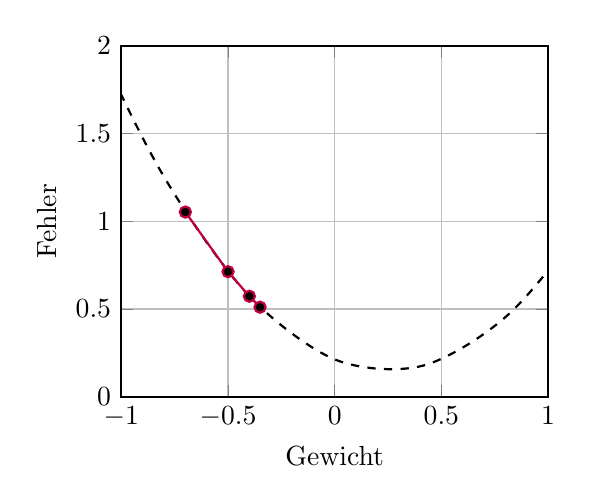
\begin{tikzpicture}
            \begin{axis}[xlabel=Gewicht,ylabel=Fehler,width=7cm,xmin=-1,xmax=1,ymin=0,ymax=2,thick,grid=both]
                \addplot[dashed,smooth] {(x-0.25)^2+0.15};
                \addplot[mark=*,draw=purple] coordinates {(-0.7,1.0525) (-0.5,0.7125) (-0.4,0.5725) (-0.35,0.51)};
            \end{axis}
        \end{tikzpicture}
        \caption{Zu niedrige Lernrate}
    \end{figure}
\end{minipage}%
\begin{minipage}{0.5\textwidth}
    \begin{figure}[H]
        \centering
        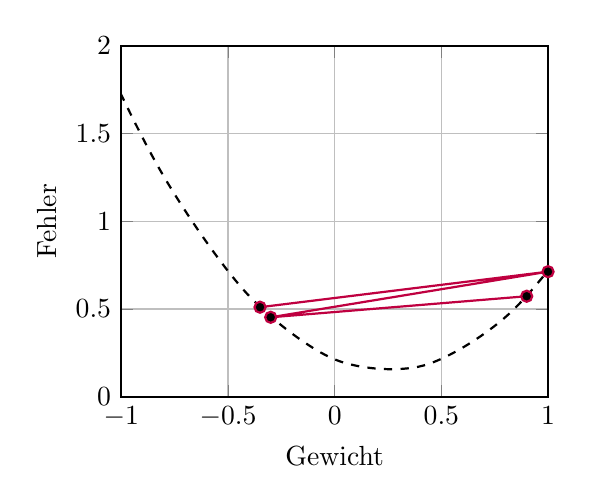
\begin{tikzpicture}
            \begin{axis}[xlabel=Gewicht,ylabel=Fehler,width=7cm,xmin=-1,xmax=1,ymin=0,ymax=2,thick,grid=both]
                \addplot[dashed,smooth] {(x-0.25)^2+0.15};
                \addplot[mark=*,draw=purple] coordinates {(-0.35,0.51) (1,0.7125) (-0.3,0.4525) (0.9,0.5725)};
            \end{axis}
        \end{tikzpicture}
        \caption{Zu hohe Lernrate}
    \end{figure}
\end{minipage}

Das Training eines neuronalen Netzes wird aufgrund der Rechenintensität und den
notwendigen Zeitaufwand für gewöhnlich nicht bis zum Optimum durchgeführt.
Stattdessen wird auf eine bestimmte Genauigkeit hingearbeitet und bei Erfüllung
dieser die erlernten Kantengewichte gespeichert und zur Wiederverwendung exportiert.